\chapter{\label{ch:data-anyl-viz}Data Analysis and Visualization}
Collecting and managing data is a key part of this project, although simply collecting data does not provide any benefit to athletes. Data analysis and visualization are essential to extract useful information from the data. This chapter will discuss the data analysis and visualization process, including cleaning of the data collected, the analysis performed, and the visualizations generated and presented as feedback to users.

\section{\label{sec:data-cleaning}Data Cleaning}
The data collection step was developed to reduce any cognitive load for users. As a result, there are a number of data sources, and therefore a number of data formats, which need to be cleaned and transformed into a uniform format for further analysis. Furthermore, some athletes might use a number of devices to track a session, so it is also necessary to match multiple session results to a given session. All the raw data from the data providers was stored throughout the project in case the data cleaning steps changed; this allowed database tables to be as small, and queryable, as possible.
\subsection{Identifying Valuable Data}
In order to begin data cleaning, it was important to understand what information was valuable. In order to do this, collected data was analysed for what information was available across each session provided, then understanding what basic analysis and feedback would be most useful to athletes. The most basic information clearly needed is the date and time of a session, what modality of session it is (row, ergometer, or other), and what type of session it is (endurance, interval, strength). These modalities and types were intentionally kept quite simple, with only three options, in order to make analysis easier to start. Next, in order to do any kind of fatigue or training impulse analysis, the duration of a session needed to be considered, along with any available heart rate or RPE information. Finally, rowers measure progress in training through mileage so a session's mileage, where appropriate, was included in this standardised model. As a result of this brief macro-analysis of the data and expected analysis results, the "Standard Exercise Model" described in the previous chapter (\autoref{tab:std_exercise_model}) was generated.

\subsection{Developing a Cleaning Process}
The data collection pipeline ingests sessions regardless of type. This required a series of functions to handle data from different providers and perform analysis on session data to appropriately classify each session, and normalise to the standard exercise model developed in the previous chapter.

\subsubsection{Identifying session modality}
The first step in cleaning data was identifying the session's modality. Was a session a row, an erg, or something else? Typically the sessions were tagged, with sessions coming from Strava being classed as "rowing", regardless of if they were on the water or on the rowing machine, causing some issues. Sessions not explicitly tagged by Strava, for example, or ingested from Concept2 were initially flagged as other. This approach, however, did result in some issues. One member of the Commercial Senior Squad, for example, uses a running watch which classifies on-the-water sessions as runs. He also happens to be an avid runner so it was necessary to analyse sessions to determine if they occurred on land or on water. As a result of this case, and the issues with differentiating on the water or on the machine "rowing" from Strava, it became clear a more developed approach was necessary to accurately identify session types. Differentiating on-the-water rows and erg sessions was much easier. In many cases, erg sessions were provided through the Concept2 API and were easily identified. On-the-water rows were typically provided through Strava and were identified by the activity type and generally the presence of GPS data. Users who did not have a GPS in the boat could manually insert sessions and the name of the session could be used to identify the modality.


\subsubsection{Identifying session type}
The next challenge in the data cleaning process was determining if a session was an endurance or interval session. Typically, the distance and duration can be used to identify a session. For erg sessions provided through the Concept2 API, distance, time, watts, and pace were included at a minimum. It is possible to differentiate endurance or interval sessions when comparing pace with other sessions from that user. The ideal session data from Concept2, though, includes highly detailed information about a session such as distance, duration, average wattage, pace, and heart rate, and detailed stroke-by-stroke data including wattage, pace, and heart rate. Many athletes, though, choose not to connect a heart rate monitor to their rowing machine, so it was necessary to match heart rate data, recorded through Polar, with the stroke data, when available. Using heart rate it is very easy to identify if an erg session is an interval or endurance session.

Identifying the type of an on the water row was more difficult. Some on-the-water sessions may be a mix of interval and endurance. A common training session for the researcher throughout this project was 10 kilometres of endurance paddling, followed by 10 kilometres of interval work. In this case, the session could be classified as an interval session. The researcher, however, would separate this into two sessions, classifying the first 10 kilometres as endurance training, considering the duration and average heart rate, and the second 10 kilometres as interval training, again considering the duration and average heart rate to calculate the training impulse. This is a clear example of the limitations of the data collected. The researcher could manually classify this session as an endurance session, but this would not be scalable. A model could be developed to classify this session, but unfortunately, not enough data was collected and classified to warrant the time needed to develop the model. As a result, the approach used to classify sessions relied on distance and average heart rate, if available. Sessions greater than 18 kilometres in distance were considered endurance sessions, then average heart rate was used to identify endurance or interval sessions below this threshold. This is a limitation of the data collected and is a clear area for future work.

Finally, strength sessions needed to be identified. When a session was ingested as a strength session this was typically already tagged. Logging strength sessions using a heart rate watch typically is not effective. Strain experienced during strength sessions rarely has a direct correlation to heart rate as cardio sessions do. Furthermore, many users did not log strength sessions using one of the supported data sources as most athletes made use of an app like TeamBuildr\footnote{\href{https://www.teambuildr.com/}{TeamBuildr} is an online strength and conditioning platform for coaches to build S\&C plans for their athletes and for athletes to track their weights sessions}, to track these sessions. As a result, strength sessions were not normally included in the training impulse analysis.  This is another clear limitation of the data collection process implemented and an area for future work. 

\section{\label{sec:data-anyl}Data Analysis}
The data collected and cleaned was then analysed to provide feedback to athletes. A number of analysis metrics were generated. Starting with basic metrics such as weekly mileage and duration, time spent in given training zones, analysis of time and mileage compelted across different modalities, and basic training load analysis. This section will discuss the approach used to generate analysis metrics for the project, and how the Standard Exercise Model was used and adapted.

\subsection{Analysis Development Methods}
Using the Standard Exercise Model developed in the previous chapter, analysis was performed. In order to generate metrics, the data available first needed to be explored. This exploration and initial analysis was done using Python, in jupyter notebooks, with the help of packages like pandas and numpy. To do this, core session information from the researchers sessions was fetched from the Standard Exercise Model table, and basic analysis performed. This included calculating weekly mileage and duration, time spent in training zones, and training impulse. Then, using the original data source, modality analysis could be refined to produce more effective feedback for athletes. This process was repeated for each analysis metric generated. Once a series of analysis metrics were generated in a Jupyter notebook, functions were developed to automate the process. These functions were then used to generate analysis metrics for all users in the database. In some cases, the analysis functions were ported to Typescript to be run directly on the client side to generate metrics based on different timeframes selected by users on the frontend. Any data that was ever interacted with was data the researcher had generated as a part of training. This was done to ensure the data was clean and accurate, and to ensure the researcher was not interacting with any sensitive data.

\subsection{Analysis Metrics Generated}
The metrics generated for analysis were based on the Standard Exercise Model developed in the previous chapter. The model was used to generate a number of analysis metrics for rowers. These metrics were then used to provide feedback for rowers in the application. The metrics generated were:
\subsubsection{Weekly mileage and duration}
Calculating weekly mileage and training duration metrics were very straightforward. Every session ingested by the platform required at a minimum duration, and if the session was a row or erg session, mileage. Using the pandas library in Python, the data was grouped by day, week, and month and the sums of mileage and duration calculated. 
This data was then used to generate a graph of weekly mileage and duration for each rower. This graph was used to track progress over time and to provide feedback to rowers on their training volume. This is a key metric for rowers to track as it is a key indicator of progress in training.
\subsubsection{Training zone mileage and duration}
Training zones were calculated using the heart rate data available for each session. The researcher used the heart rate data to calculate the time spent in each training zone. This was done using the average heart rate described in the Standard Exercise Model. Athletes were asked to input their maximum and resting heart rates, which were used to determine training zones based on HR ratio. The time and mileage spent in each zone was calculated similarly to the weekly mileage and duration metrics. A pandas pivot table was used to group the data by zone and sum the mileage and duration. This data was then included in the daily, weekly, and monthly dataframes passed on to the further analysis functions and in turn the visualisation functions. Understanding how much time is spent in each zone throughout the week allows rowers to ensure they are training effectively. If they are following a polarised or threshold training plan, this metric can be used to ensure they are executing the correct split of training zones.
\subsubsection{Modality analysis}
Modality analysis was performed to understand how much time was spent on the water versus on the erg. This was done by grouping the data by modality and summing the mileage and duration. This data was then included in the daily, weekly, and monthly dataframes passed on to the further analysis functions and in turn the visualisation functions. This metric is important for rowers to track as it can indicate if they are spending too much time on the erg or on the water. This can be important for rowers to track as it can indicate if they are at risk of injury from overtraining on the erg or if they are not spending enough time on the water to develop their technique. When looking at a rower as a coach, more time on the water can lead to more efficiency in technique. If a rower finds they are not performing as expected on the water, they may need to spend more time on the water to develop their technique. Additionally, when considering features for a model to predict injury, extensive time on the erg may potentially be a factor. This can be a potential issue particularly if a rower changes from doing no erg work to almost exclusively erg work. Deeper analysis can explore a wider range of potential modalities, such as running and cycling, and exploring how these modalities interact with rowing training and performance.
\subsubsection{Training load analysis}
The most in-depth analysis performed was training impulse analysis. As described in the training quantification subsection (\autoref{sec:quant-training}), training impulse is an approximation of the strain a training session places on an athlete. For this project, it is calculated by multiplying the duration of a session by the average heart rate of the session. This is a simple way to quantify the stress a session places on an athlete. The training impulse of a session can be used to calculate the training load of a week, month, or year. This can be used to track fatigue and fitness over time. Due to the limitations in data available, fitness and fatigue scores for rowers were not calculated, this will be discussed further in the Data Analysis section of the Discussion Chapter (\ref{sec:data-anyl-diss}).
Each session with heart rate data available had a training impulse (\texttt{trimp}) value generated. This value could then be used to calculate acute and chronic workload, which in turn were used to calculate the acute chronic workload ratio (ACWR) a rower was experiencing. Presenting this analysis to rowers can indicate if they are at risk of injury by overtraining, as a result of increasing load, or undertraining for a period of time beyond a productive taper. This is a key metric for rowers to track and is a key part of the feedback provided to rowers in the application.

\section{\label{sec:data-viz}Data Visualisation}
The data visualisation built upon the analysis done, representing the outcomes of the analysis graphically making them easier to understand at-a-glance. To develop visualisations, Python was once again used in a Jupyter notebook, with the help of the matplotlib library to generate plots. The plots generated in the Jupyter notebook were then mostly ported to Typescript, using the Plotly.js library, to be used in the application. This section will discuss the approach used to generate visualisations for the project, how the analysis metrics discussed in the previous section were used and adapted, and the process for bringing visualisations to the frontend.

\subsection{Visualisation Development Methods}
As a result of the analysis steps taken, a set of pandas DataFrames were generated, these could be used to easily generate basic plots for visualisations. In isolation though, certain plots were not as useful as they could be. For example, a bar plot of daily training impulses is not particularly useful, especially given the arbitrary nature of the units it is measured in. A more useful plot may overlay acute workload, chronic workload, and ACWR lines plots to add some more useful context for a rower. This iterative approach of visually exploring the data, determining if a metric in isolation was useful, or finding a suitable pairing of metrics to plot together, was used to generate the visualisations for the project. Each plot generated was made into a function which including any data transformations necessary to generate the visualisation. These functions were then ported to Typescript to generate the graphs in the application, leveraging the Plotly.js library.

\subsection{Visualisations Generated}
This subsection discusses the visualatisations generated. All the data used is from the researchers training and is up to date as of April 7, 2024.

\subsubsection{Acute, Chronic, TRIMP, ACWR Chart}

\begin{figure}[htbp]
  \centering
  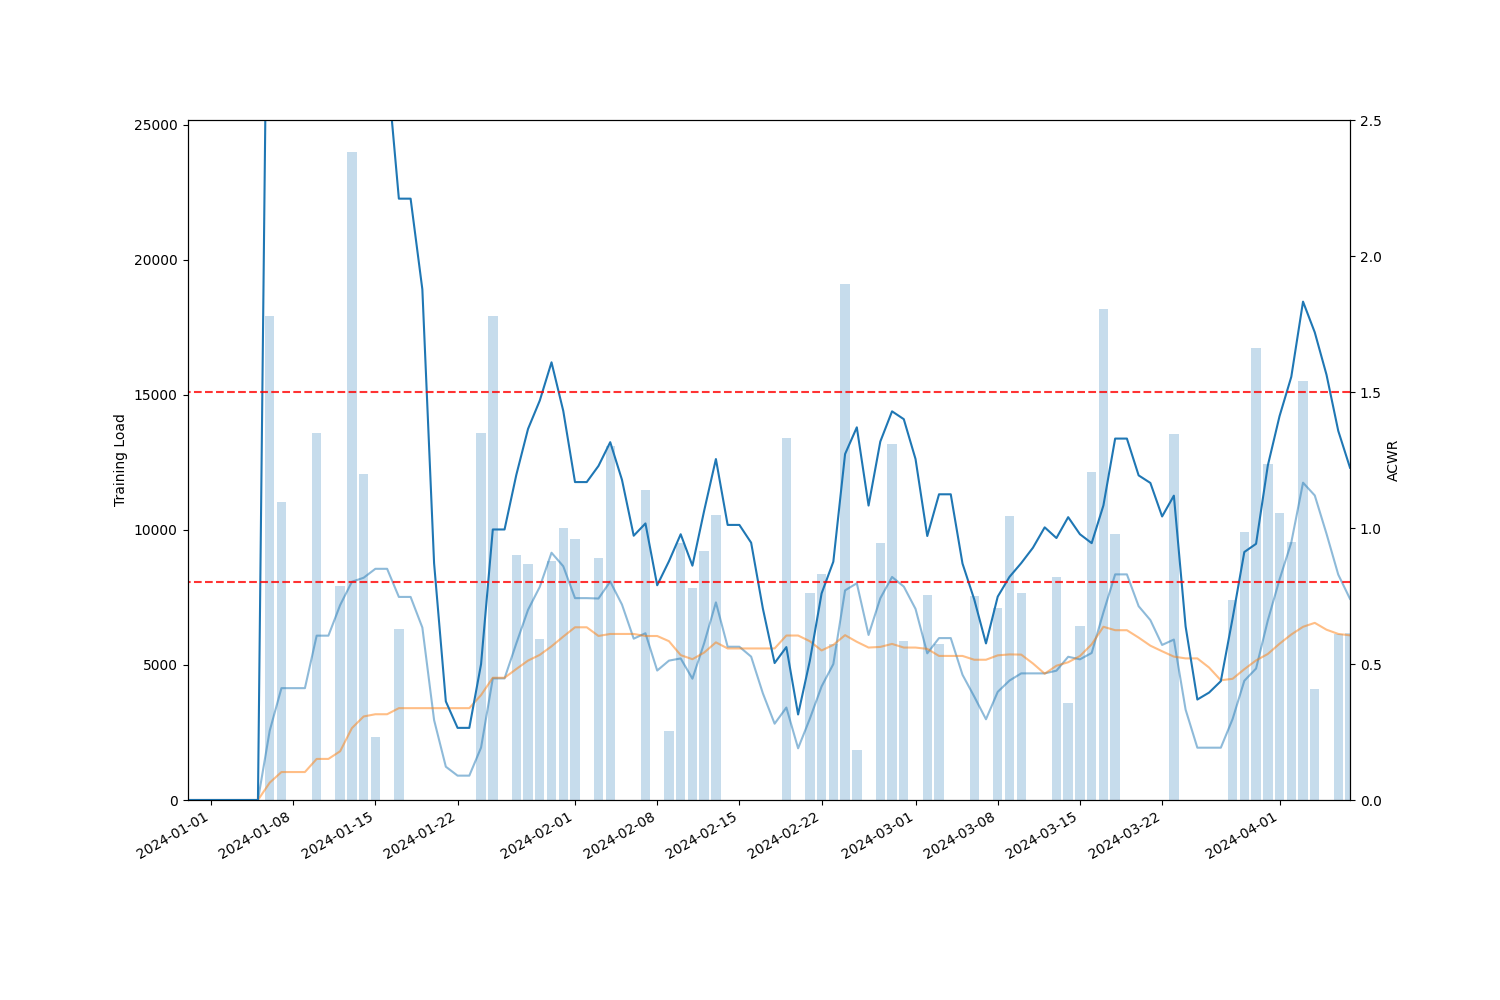
\includegraphics[width=\linewidth]{figures/acwr.png}
  \captionsetup{justification=centering}
  \caption[ACWR Chart]{\label{fig:acwr}The Acute, Chronic, TRIMP, ACWR chart}
\end{figure}
The primary chart implemented on the frontend is the ACWR chart. The version shown in \autoref{fig:acwr}, is generated from the Jupyter notebook used to develop visualisations, using the researchers training data on April 7, 2024. This chart looks at a roughly 100 day period from December 28 to April 7, 2024. During this period the researcher recovered from an ankle sprain, and two periods of illness, accounting for gaps in training (trimp bars) and the erratic nature of the ACWR line.

This chart displays daily training impulse (arbitrary units), as bars, acute and chronic workload (arbitrary units), as low opacity lines (acute workload in blue, chronic workload in orange), and ACWR on a second axis (solid blue line). This chart is useful for rowers to track their training load over time and to ensure they are not at risk of injury from overtraining. The two red lines overlayed on the ACWR axis at 0.8 and 1.3 indicate the optimal training load range. 

When implementing this chart in the frontend, a datepicker was added to allow users to explore how their training over different time periods was balanced. This resulted in a more interactive chart, allowing users to explore their training load over time. This chart was the most complex to implement, as it required the most data to be passed to the frontend, and given the multi axis nature of the data, it was not possible to create a generalised, reusable, chart component.

\subsubsection{Weekly training overview}

\begin{figure}[htbp]

    \centering
    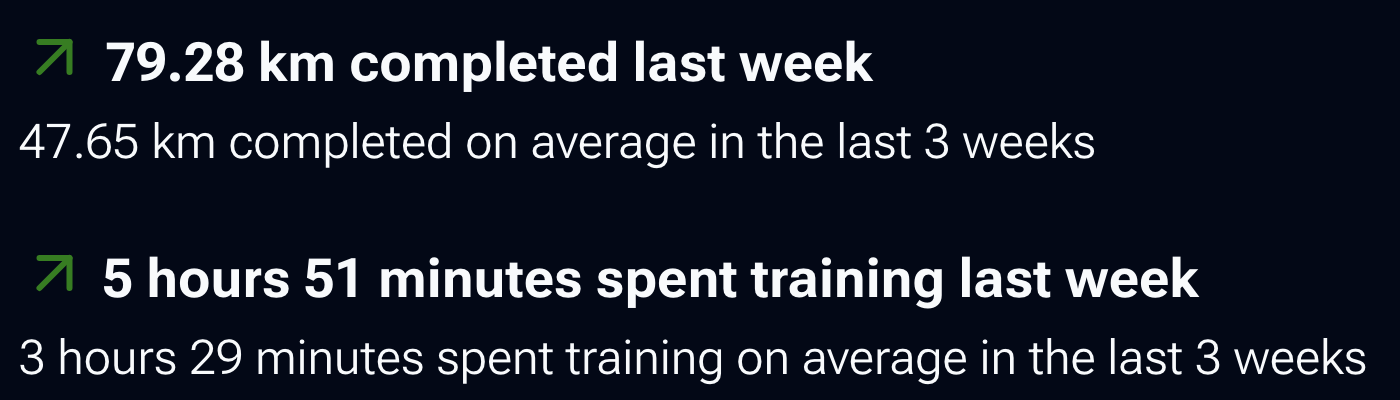
\includegraphics[width=0.75\linewidth]{figures/trainingOverviewWidget.png}
    \captionsetup{justification=centering}
    \caption[Weekly Training Overview]{\label{fig:weeklyTrainingOverview}The weekly training overview widget, comparing the last weeks mileage and training time to the average of the previous 3 weeks} 
\end{figure}

The weekly training overview widget (\autoref{fig:weeklyTrainingOverview}) was the only visualisation not initially developed in the Jupyter notebook, a text version was created, but due to styling needed it made more sense to develop this directly in Typescript. This visualisation shows the mileage and training duration for the last week, which updates each day, and compares that with the rolling average of the last 3 weeks. This chart is useful for rowers to track their progress over time and to ensure they are hitting their weekly mileage targets. This visualisation was the simplest to implement, as it required the least data to be passed to the frontend, and was an easy to generalise component in react.


\subsubsection{Modality and Zone Donuts}

\begin{figure}[htbp]
  \centering
  \begin{minipage}[c]{0.45\linewidth}
    \centering
    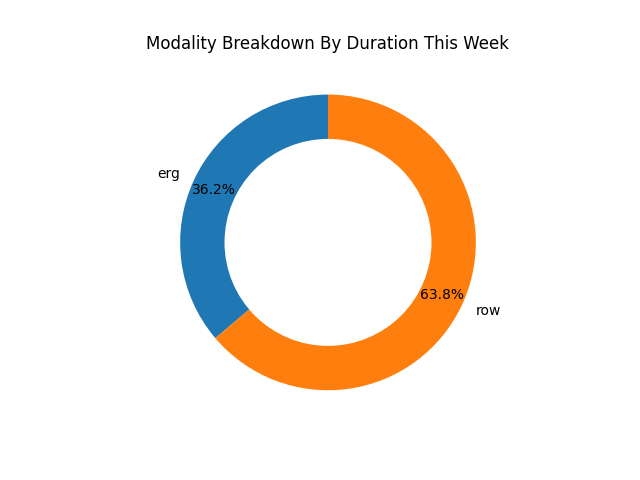
\includegraphics[width=\linewidth]{figures/durationDonut.png}
    \captionsetup{justification=centering}
    \caption[Duration Donut]{\label{fig:durationDonut}A donut graph showing the distribution of training duration across different modalities}
  \end{minipage}
  \begin{minipage}[c]{0.45\linewidth}
    \centering
    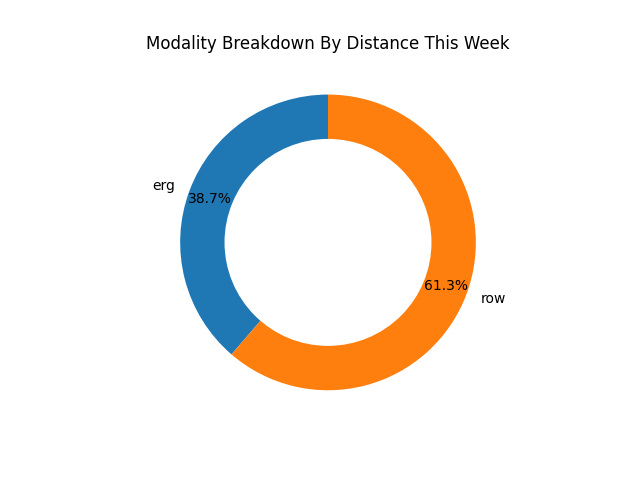
\includegraphics[width=\linewidth]{figures/distanceDonut.png}
    \captionsetup{justification=centering}
    \caption[Distance Donut]{\label{fig:distanceDonut}A donut graph showing the distribution of training distance across different modalities}
  \end{minipage}
\end{figure}
Rowers tend to split training across a number of modalities, most training is completed either on the erg or on the water. The donut charts in \autoref{fig:durationDonut} and \autoref{fig:distanceDonut} show the distribution of training duration and distance across different modalities. The data shown is the training distribution for the week starting on April 1, 2024. One draw back of the data collection and cleaning implemented for this project was the limited number of training modalities logged. Including modalities such as cycling, running and swimming could provide a more complete picture of training modality distribution, particularly in the winter season when mileage, in any form, is the target.

This visualisation is useful for rowers to track as it can indicate if they are spending too much time in the "other" category currently supported by the platform rather than on the erg or on the water. Furthermore, rowers with less rowing experience might look to optimise time spent on the water to improve their technique.

This visualisation was relatively easy to implement, Plotly.js library being quite lenient with how data could be passed to the donut chart. This visualisation was also generalised to be reusable, so it could be used for both duration and distance data.

\subsubsection{Modality Duration and Distance Charts}

\begin{figure}[htbp]
  \centering
  \begin{minipage}[c]{0.45\textwidth}
    \centering
    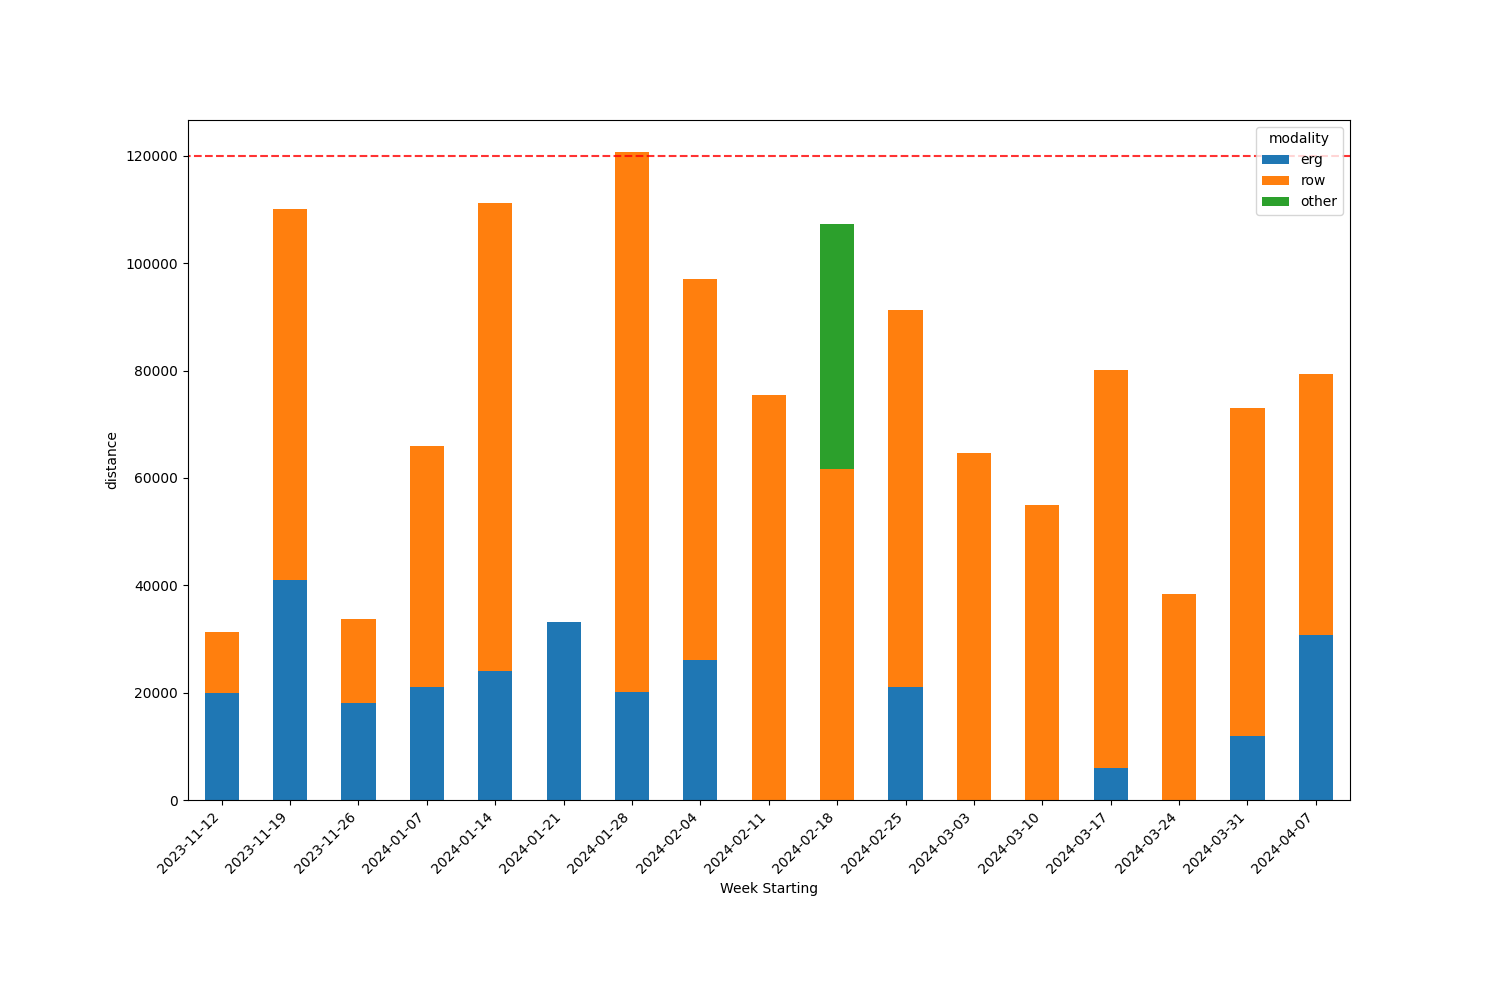
\includegraphics[width=\linewidth]{figures/distanceVsMod.png}
    \captionsetup{justification=centering}
    \caption[Distance by Modality]{\label{fig:distanceVsMod}A stacked bar chart showing the weekly distance completed across different modalities}
  \end{minipage}
  \begin{minipage}[c]{0.45\textwidth}
    \centering
    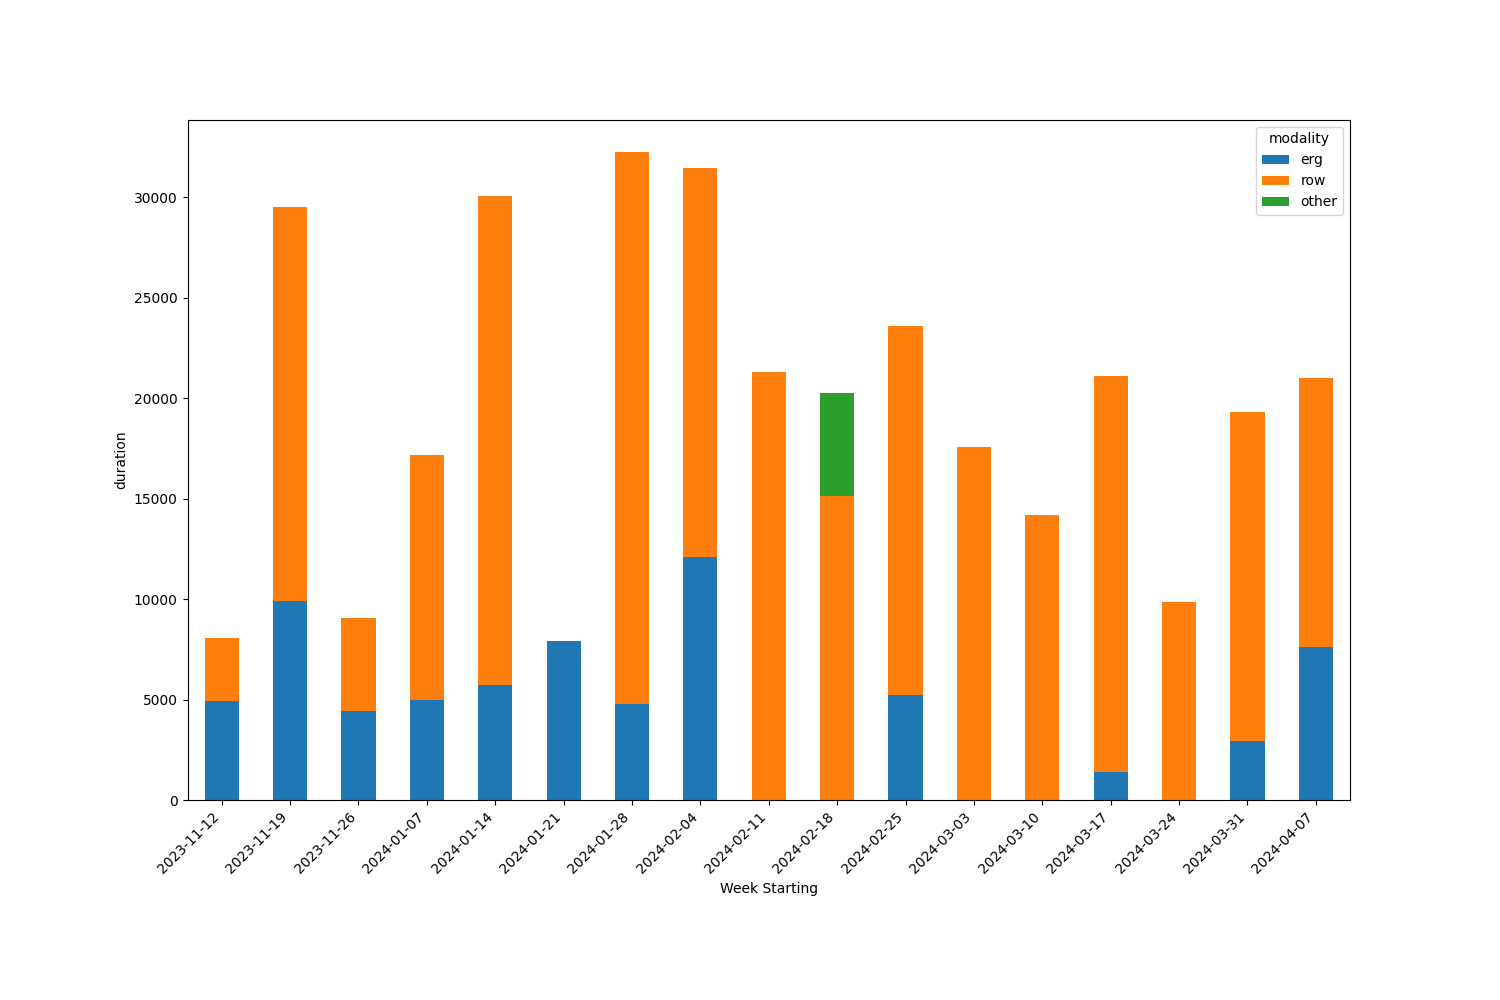
\includegraphics[width=\linewidth]{figures/durationVsMod.png}
    \captionsetup{justification=centering}
    \caption[Duration by Modality]{\label{fig:durationVsMod}A stacked bar chart showing the weekly duration completed across different modalities}
  \end{minipage}
  \caption*{Full sized versions of these charts are available in the appendix}
\end{figure}

The stacked bar charts in \autoref{fig:distanceVsMod} and \autoref{fig:durationVsMod} show the weekly distance and duration completed across different modalities since the second week of November, 2023. This chart only includes weeks where any training was completed, so gaps that would exist as a result of illness or injury are not shown. Similar to the donut charts, this provides rowers with a snapshot of how they are distributing their weekly mileage, and time. If a significant difference in how a given week's time and distance is observed, a rower can prioritise a certain modality to balance their training. This is particularly useful for rowers who may be particularly busy, as they can prioritise erg sessions which are typically a shorter time-commitment for the same mileage. These visualisations can also include overlays, such as the dotted red line in thd duration chart (\autoref{fig:durationVsMod}). This dotted line deliniates the weekly 120km target the researcher has set, again due to injury and illness this target has not been hit during many of the weeks of training shown. Rowers could also select to include a duration target as well.

This visualisation did not make it to the frontend as there were a number of formatting and styling issues encountered. With more time, this visualisation could be implemented, but it was not a priority for the project.

